\documentclass[12pt]{amsart}
\usepackage{fullpage}
\usepackage{pbox}
\usepackage{graphicx}
\usepackage{booktabs} % Top and bottom rules for table
\usepackage{amsfonts, amsmath, amsthm, amssymb}
\usepackage{longtable,array,color,xcolor}
\usepackage[colorlinks = true,
            urlcolor  = blue]{hyperref}
\usepackage{verbatim}
\usepackage{enumerate}
\usepackage{lscape}
\newcommand\narrowstyle{\SetTracking{encoding=*}{-50}\lsstyle}

\setlength{\parindent}{0pt}

\begin{document}
\flushright
Name:\underline{\hspace{5cm}}
\title{Math 320: Quiz 4}
\maketitle

\begin{enumerate}
\item (3 points) Let $f(x) = x^2e^{-x}$. 
\begin{enumerate}
\item Compute the first and second derivatives $f'(x)$ and $f''(x)$

\vspace{3cm}

\item Based on this computation, list the local optima of $f(x)$
and whether each point is a maximum or minimum. 

\vspace{4cm}

\item Are these points global optima?
\end{enumerate}

\vspace{4cm}

\item Let $g(x) = x^3 - x^2 - 3x - 1$.

\begin{enumerate}
\item We would like to minimize the value of $g(x)$
between $0$ and $2$. Suppose our initial root estimate is $x=1$.
What is the equation (in the form $y = ax^2 + bx + c$) 
for the parabola $P$ that intersects the graph of $g(x)$ at 
each of these $x$-values.

\vfill
\pagebreak

\item Where does $P$ attain its minimum?

\end{enumerate}

\vspace{4cm}

\item Suppose $A$ is a matrix describing a map from $\mathbb{R}^2$ to 
$\mathbb{R}^2$
sending the solid vector $(1,0)$ and the dashed vector $(0,1)$ to
the corresponding vectors in the picture at right. 

\vspace{5mm}

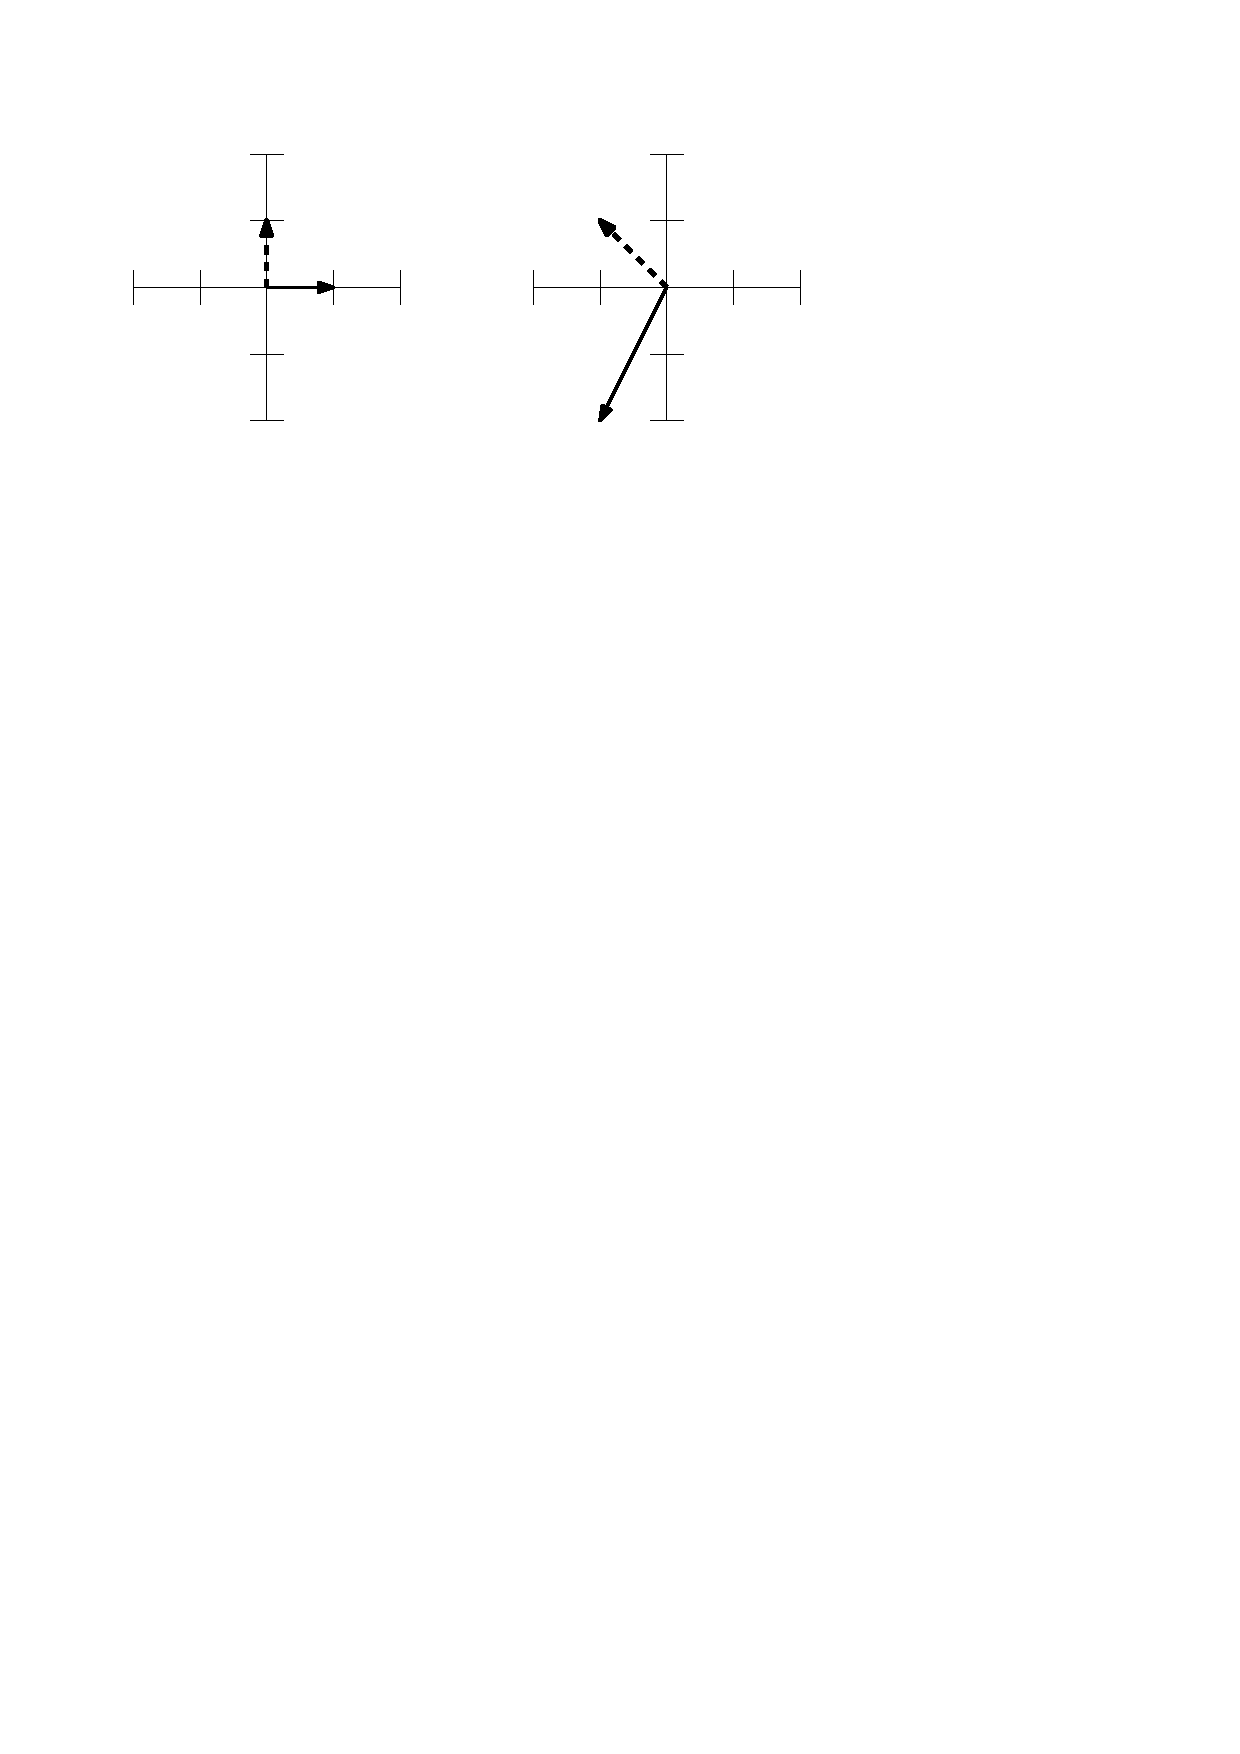
\includegraphics{q4p3.pdf}

\begin{enumerate}
\item Please write $A$ as a $2\times 2$ matrix.

\vspace{4cm}
\item Evaluate the determinant of $A$.
\end{enumerate}

\end{enumerate}

\end{document}
